% $Id$
% ---------------------------------------------------------------------------
%
% Copyright (c) 2008 Interlegis
%
% Permission is granted to copy, distribute and/or modify this
% document under the terms of the GNU Free Documentation License,
% Version 1.2 or any later version published by the Free Software
% Foundation; with no Invariant Sections, no Front-Cover Texts, and no
% Back-Cover Texts.  A copy of the license is included in the section
% entitled "GNU Free Documentation License". If not, see
% <http://www.gnu.org/licenses/>.
%

\documentclass[a4paper,12pt]{article}
\textheight 22.5cm
\usepackage[brazil]{babel}      % suporte ao portugues brasil
\usepackage[utf8]{inputenc}     % Codificacao dos caracteres (use a
                                % codificacao latin1 caso seu
                                % sistema/editor nao suporte utf8).
\usepackage[T1]{fontenc}
\usepackage{indentfirst}        % indenta o primeiro paragrafo 
\usepackage{graphicx}           % uso para imagens
\usepackage{dsfont}             % fonte

\usepackage{fancyhdr}           % permite alterar o cabecalho
\pagestyle{fancy}               % configura o estilo padrao

\usepackage{verbatim}

% $Id$
% ---------------------------------------------------------------------------
%
%  This is part of the SIGI.
%  Copyright (C) 2008 Interlegis
%  See the file relatorio.tex for copying conditions.
%

\newcommand{\titulo}{Produto IV}
\newcommand{\subtitulo}{Sistema de Informações Gerenciais do Interlegis}
\newcommand{\autor}{Guilherme Mesquita Gondim}
\newcommand{\numcontrato}{2008/000471} % Número do contrato caso seja
                                        % consultor.

%
% Local variables:
%   mode: flyspell
%   TeX-master: "relatorio.tex"
% End:
%
                % novos comandos

\usepackage[pdftex,%            % formatacao no PDF
pdfauthor={\autor},%
pdftitle={\titulo \ - \subtitulo},%
]{hyperref}
\hypersetup{backref=true,pdfpagemode=UseOutlines,colorlinks=true,
  breaklinks=true,hyperindex,linkcolor=blue,anchorcolor=black,
  citecolor=blue,filecolor=magenta,menucolor=red,pagecolor=red,
  urlcolor=cyan,bookmarks=true,bookmarksopen=true,pdfpagelayout=SinglePage,
  pdfpagetransition=Dissolve}

\begin{document}
% $Id$
% ---------------------------------------------------------------------------
%
%  This is part of the SIGI.
%  Copyright (C) 2008 Interlegis
%  See the file relatorio.tex for copying conditions.
%

\lhead {
  \setlength{\unitlength}{5mm} 
  \begin{picture}(0,0) 
    
\includegraphics[scale=0.65]{imagens/cabecalho.pdf} 
  \end{picture} 
}
\chead{}
\rhead{}
\renewcommand{\headrulewidth}{0pt}

%
% Local variables:
%   mode: flyspell
%   TeX-master: "relatorio.tex"
% End:
%

% $Id$
% ---------------------------------------------------------------------------
%
%  This is part of the SIGI.
%  Copyright (C) 2008 Interlegis
%  See the file relatorio.tex for copying conditions.
%

\textsf{\vspace{6cm}}
\begin{center}
  \noindent
  \large{
    \textbf{\titulo}
  } \\

  \Large{
    \textbf{\subtitulo}
  } \\
  \large{
    \textbf{APO-CASA}
  }

  \vspace{9cm}

  \large{
    \textbf{\autor}\\
    \textsf{Contrato N$^{\circ}$: \numcontrato}\\
  }
\end{center}
\cfoot{}

%
% Local variables:
%   mode: flyspell
%   TeX-master: "relatorio.tex"
% End:
%


% configura o rodape do conteudo pre-textual para numeros romanos
\clearpage
\cfoot{\thepage}
\setcounter{page}{1}
\pagenumbering{Roman}

\tableofcontents
\listoffigures

% configura o rodape das paginas de conteudo para numeros convencionais
\clearpage
\setcounter{page}{1}
\pagenumbering{arabic}

% conteudo
%
%  This is part of the SIGI.
%  Copyright (C) 2008 Interlegis
%  See the file relatorio.tex for copying conditions.
%

\section{Introdução}
Este documento detalha as atividades desenvolvidas durante a quarta
etapa do projeto de desenvolvimento do Sistema de Informações
Gerenciais do Interlegis (SIGI).

A quarta etapa consiste nos treinamentos de utilização da tecnologia
``Django Web Framework'', aplicada no desenvolvimento do SIGI, e sobre
o uso do SIGI.

As seções \ref{sec:django}, \ref{sec:sigidev} e \ref{sec:sigiuso}
apresentam, respectivamente, os objetivos e conteúdo programático do
treinamento em Django, desenvolvimento para o SIGI e uso do SIGI.

A seção \ref{sec:bib} possui a bibliografia necessária para o
treinamento em desenvolvimento web com Django e do SIGI.

Na seção \ref{sec:anexos}, estão anexadas a documentação técnica
produzida para o SIGI.

%
% Local variables:
%   mode: flyspell
%   TeX-master: "relatorio.tex"
% End:
%

%
%  This is part of the SIGI.
%  Copyright (C) 2008 Interlegis
%  See the file relatorio.tex for copying conditions.
%

\section{Informações gerais}
\label{sec:info}

\subsection{SIGI}

O \textbf{SIGI} é um projeto para um Sistema de Informações Gerenciais
do \emph{Interlegis}, escrito na linguagem de programação Python com o
framework para desenvolvimento web Django.

\begin{description}
\item[Página do projeto:]
  http://colab.interlegis.gov.br/wiki/ProjetoSigi
\item[Repositório de código (Subversion):]
  http://repositorio.interlegis.gov.br/SIGI
\end{description}


\subsection{Características}
Lista das principais características do SIGI:

\begin{itemize}
\item Serviço web cliente/servidor, podendo ser disponibilizado tanto
  na internet quanto na intranet;
  
\item Multi-plataforma;
  
\item Baseia-se na interface de administração nativa do Django\\
  (\verb|django.contrib.admin|);
  
\item Gerencia convênios, equipamentos e inventários, serviços
  prestados e composição de Mesas Diretoras das Casas Legislativas;

\item Autenticação no sistema baseada em usuários e grupos, com perfis
  diferentes;

\item Geração de relatórios.
\end{itemize}

\subsection{Licença de Uso}
O SIGI é disponibilizado como \emph{software livre}, isto significa
que você pode redistribuí-lo e/ou modifica-lo dentro dos termos da
Licença Pública Geral GNU (GPL) como publicada pela Fundação do
Software Livre (FSF); na versão 3 da Licença, ou (na sua opinião) em
qualquer versão mais recente.

%
% Local variables:
%   mode: flyspell
%   TeX-master: "relatorio.tex"
% End:
%

%
%  This is part of the SIGI.
%  Copyright (C) 2008 Interlegis
%  See the file relatorio.tex for copying conditions.
%

\section{Organização do sistema}
\label{sec:org}

\subsection{Listagem do conteúdo dos diretórios}
\verbatiminput{../arquivos/tree.txt}

\subsection{Descrição dos arquivos e diretórios}
\begin{description}
\item[COPYING:] Arquivo com a licença do sistema (GPLv3).

\item[LEIA-ME/README:] Contém informações do sistema, nota de
  copyright e instruções de instalação.

\item[devel.db:] Base de dados SQLite utilizada para desenvolvimento
  do sistema.

\item[docs/:] Diretório com toda documentação escrita para o sistema
  (relatórios, manual de instalação, casos de uso, esquema de base de
  dados, etc).

\item[etc/:] Diretório com arquivos variados: configuração do Apache,
  \textit{patchs} de códigos, etc.

\item[media/:] Diretório com arquivos estáticos e de mídia do sistema
  (imagens, CSS, javascripts).

\item[sigi/:] Pacote Python do sistema.

\item[sigi/admin/:] Pacote de código relacionado com a aplicação
  \verb|admin| do Django (\verb|django.contrib.admin|).

\item[sigi/apps/:] Pacote de aplicações do sistema, maiores
  informações na Seção \ref{sec:apps}.

\item[sigi/settings.py:] Configurações padrões do sistema.

\item[sigi/local\_settings.template:] Exemplo de configurações locais
  do sistema (pertinentes à instalação). Deverá ser copiado para
  \verb|sigi/local_settings.py| para sua utilização.

\item[sigi/locale/:] Diretório com localização local do projeto.

\item[sigi/manage.py:] Script de gerenciamento do projeto, gerado pelo
  framework Django.

\item[sigi/templates/:] Diretório com templates HTML do Django.

\item[sigi/urls.py:] Modulo de configuração de URLs.
\end{description}

\subsection{Descrição das aplicações}
\label{sec:apps}
O SIGI é composto de algumas aplicações Django, cada uma com um
propósito bem definido.

Uma aplicação Django é um pacote Python modular, podendo ser
reaproveitado em outros projetos.

Algumas aplicações possuem algum nível de relacionamento com as
outras. A Seção \ref{sec:rel} demonstra o relacionamento entre essas
aplicações.

Segue descrição de cada aplicação:

\begin{description}
\item[sigi.apps.casas:]
  Gerência de Casas Legislativas.

\item[sigi.apps.contatos:]
  Gerência de Contatos do Interlegis com Casas Legislativas,
  fornecedores de equipamentos, serviços e etc.

\item[sigi.apps.convenios:]
  Convênios do Interlegis com as Casas Legislativas.

\item[sigi.apps.inventario:]
  Inventário de equipamentos disponibilizados pelo Interlegis para as
  Casas Legislativas.

\item[sigi.apps.mesas:]
  Composição das Mesas Diretoras das Casas Legislativas.

\item[sigi.apps.parlamentares:]
  Gerência de Parlamentares.

\item[sigi.apps.servicos:]
  Serviços prestados às Casas Legislativas conveniadas ao Interlegis.
\end{description}

\subsubsection{Relacionamento entre as aplicações}
\label{sec:rel}

A Figura \ref{fig:apps} demonstra o relacionamento entre as
aplicações e seus \emph{models}.

Uma seta direcional representa uma relação \textit{muitos para
  um}. Uma seta bidirecional representa uma relação \textit{muitos
  para muitos}.

A seta pontilhada representa uma relação genérica, como descrito na
documentação do Django:\\
http://docs.djangoproject.com/en/dev/ref/contrib/contenttypes/\#id1

\begin{figure}[p]
  \centering
  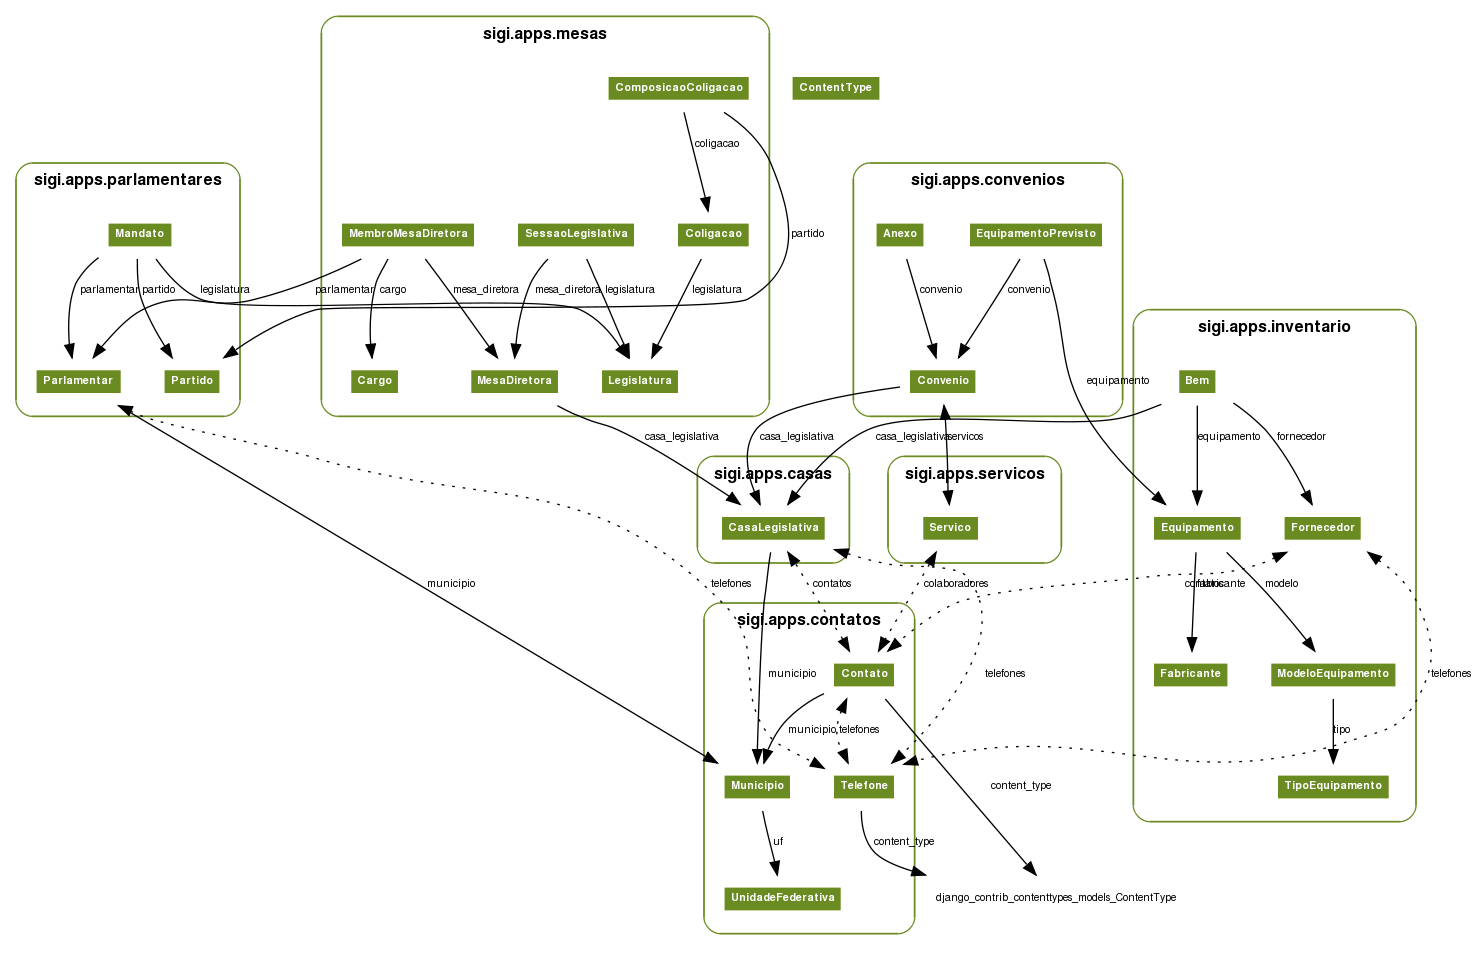
\includegraphics[angle=90,width=130mm]{../imagens/apps.png}
  \caption{Relacionamento entre as aplicações}
  \label{fig:apps}
\end{figure}


%
% Local variables:
%   mode: flyspell
%   TeX-master: "relatorio.tex"
% End:
%

%
%  This is part of the SIGI.
%  Copyright (C) 2008 Interlegis
%  See the file relatorio.tex for copying conditions.
%

\section{Atividades no repositório de código do sistema}
\label{sec:atividades}

O sistema foi desenvolvido utilizando o Sistema de Controle de Versão
Subversion. O repositório do código pode ser encontrado em:\\
http://repositorio.interlegis.gov.br/SIGI/

\footnotesize
\verbatiminput{../arquivos/svn-log.txt}

%
% Local variables:
%   mode: flyspell
%   TeX-master: "relatorio.tex"
% End:
%


\end{document}
